\documentclass[11pt]{article}
\usepackage{fullpage}
\usepackage{hyperref}
\usepackage{amssymb}
\usepackage{spalign}
\usepackage{amsmath}
\usepackage{framed}

\renewcommand{\familydefault}{\sfdefault}
\usepackage{sfmath}
\newcommand{\tb}{\textbf}

\newcommand{\R}{\mathbb{R}}

\hbadness=99999

\hypersetup{
    colorlinks,
    citecolor=black,
    filecolor=black,
    linkcolor=black,
    urlcolor=black
}
\urlstyle{urlcolor=blue}
\usepackage{graphicx}
\graphicspath{{./images/}}
\setcounter{tocdepth}{2}

\renewcommand{\contentsname}{Table of Contents}
\title{Linear Algebra Reference}
\author{Sidharth Baskaran}

\begin{document}
\maketitle

\begin{center}
    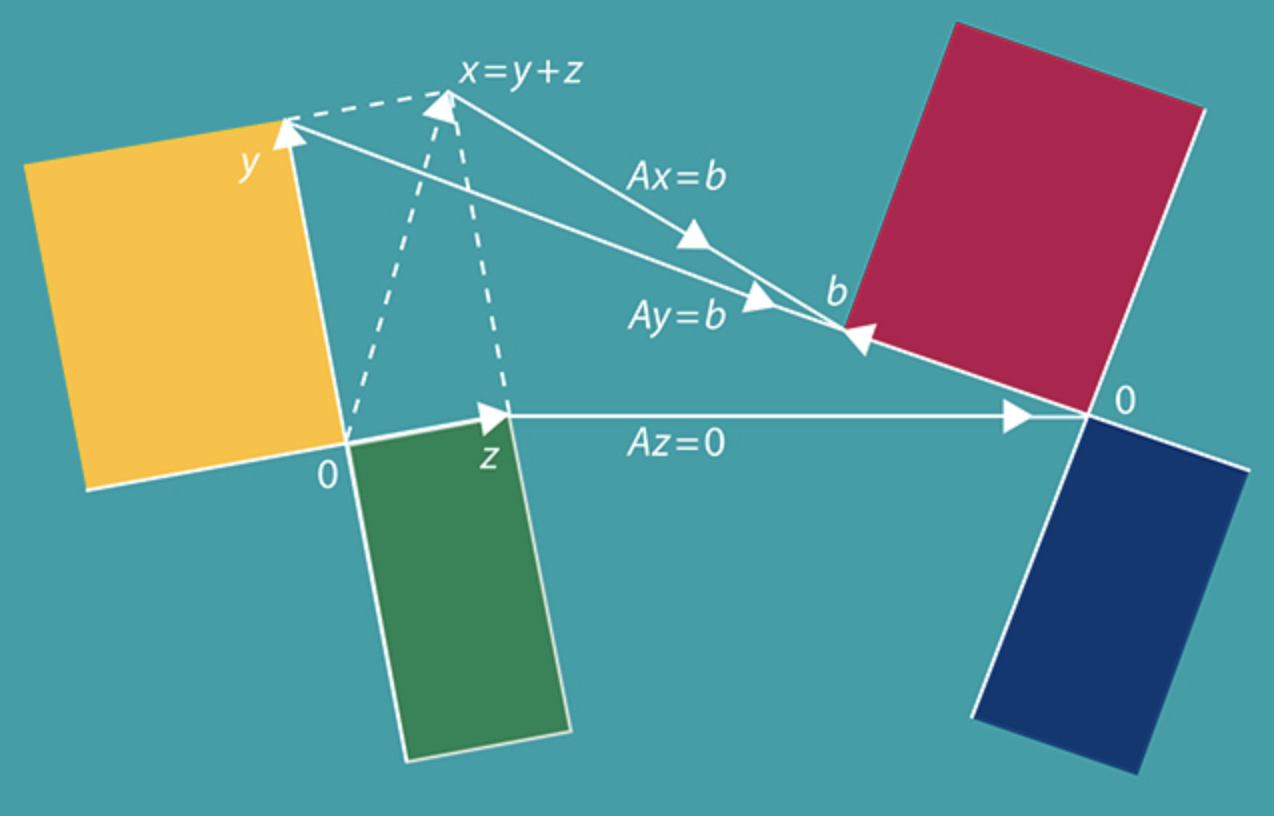
\includegraphics[scale=0.3]{cover.png}
\end{center}

\tableofcontents
\newpage
% -------------------------------------

\section{Row and Column Picture}
\subsection{Row picture}

Involves viewing matrix as linear equations graphed on a line or plane. Take the example $A\vec{x}=\vec{b}$ below:

\[\begin{bmatrix}
        1&2&3\\
        3&4&5\\
        4&5&6
    \end{bmatrix}
    \begin{bmatrix}
        x\\y\\z
    \end{bmatrix}
    =
    \begin{bmatrix}
        8\\9\\10
    \end{bmatrix}
\]

This can be viewed as the following system:

\[
    \spalignsys{
    1x + 2y + 3z = 8 ;
    3x + 4y + 5z = 9 ;
     4 + 5y + 6z = 10
    }
\]

\subsection{Column picture}

Involves viewing this setup as a linear combination of column vectors. Take $A\vec{x}=\vec{b}$ again:

\[
    x\begin{bmatrix}
        1\\3\\4
    \end{bmatrix}
    +y\begin{bmatrix}
        2\\4\\5
    \end{bmatrix}
    +z\begin{bmatrix}
        3\\5\\6
    \end{bmatrix}
    =
    \begin{bmatrix}
        8\\9\\10
    \end{bmatrix}.
\]

\subsection{Visualization in Space and Solutions}

\subsubsection{2D space}

In $\R^2$, the equations form a line. Independent column vectors means infinite linear combinations of these to get
a set of $\vec{b}$ in $\R^2$. If one column vector is dependent on another, they are parallel and various
combinations of $\vec{b}$ are on a line.

\subsubsection{3D space}

The equations form a plane in $\R^3$. If column vectors independent, infinite linear combination of $\vec{b}$
exist in 3D space. If one vector is a scaled combination of another and the third is independent, then solutions lie
on a line. If all three are interdependent, the solution is on a line.


\section{Matrix Multiplication}
\subsection{Row and Column Swapping}

Can define elementary row operations in the identity matrix.

\subsubsection{Swapping rows}

\[
    \begin{bmatrix}
        0&1\\
        1&0
    \end{bmatrix}
    \begin{bmatrix}
        a&b\\
        c&d
    \end{bmatrix}
    =
    \begin{bmatrix}
        c&d\\
        a&b
    \end{bmatrix}
\]

Modifier $B$ is always on \textbf{left}.

\subsubsection{Swapping columns}

\[
    \begin{bmatrix}
        a&b\\
        c&d
    \end{bmatrix}
    \begin{bmatrix}
        0&1\\
        1&0
    \end{bmatrix}
    =
    \begin{bmatrix}
        b&a\\
        d&c
    \end{bmatrix}
\]

Modifier $B$ is always on \textbf{right}.

\subsection{Elimination steps}

Performing elimination:

\[E_{2,1}A+E_{3,2}A=(E_{2,1}E_{3,2})A=U\]

Elimination algorithm:
\begin{itemize}
    \item $E_{2,1}$ is the pivot. Swap with $R_2$ if 0 (and $(2,1)$ is nonzero).
    \item $E_{3,2}$ involves getting $(2,2)$ as a pivot assuming nonzero to get $(3,2)$ as 0
    \item Result is invertible and non-singular, where $U$ is upper-triangular
\end{itemize}

Matrix multiplication is not necessarily commutative but always associative.

\subsection{Matrix Multiplication Facts}

If $A$ is an $m\times n$ matrix and $B$ is $n\times p$, then $AB=C$ must be $m\times p$.
Standard method would be to take dot products by row and column. By column: Columns of $C$ are combinations of columns
of $A$. By row: Rows of $C$ are combinations of rows of $B$.

\subsection{Example (Row)}

\[
    \left[\begin{array}{ll}
        2 & 7 \\
        3 & 8 \\
        4 & 9
        \end{array}\right]\left[\begin{array}{ll}
        1 & 6 \\
        0 & 0
        \end{array}\right]=\left[\begin{array}{l}
        2 \\
        3 \\
        4
        \end{array}\right]\left[\begin{array}{ll}
        1 & 6
        \end{array}\right]+\left[\begin{array}{l}
        7 \\
        8 \\
        9
        \end{array}\right]\left[\begin{array}{ll}
        0 & 0
    \end{array}\right]
\]

\section{Factorization into A=LU}
\subsection{Notation}

$E_{21}$ is the location at row 2 and column 1, used to eliminate this value.

\subsection{Inverse}

\[AA^{-1}=I=A^{-1}A\]

Matrix multiplication is not commutative:

\[\left(A B^{-1}\right)\left(B A^{-1}\right)=A I A^{-1}=I\]

Transpose inverse fact:

\[\boxed{(A^{-1})^TA^T=I}\]

\subsection{Concept}

Given $E_{21}A=U$, where $U$ is upper-triangular, $E^{-1}_{21}A=E^{-1}_{21}U$ gives:

\[\boxed{A=LU\text{ where }L=E^{-1}_{21}}\]

\section{Linear Transformations}
\subsection{Rules and Notation}

Domain is the input space and codomain is the output space.

\begin{itemize}
    \item $T(\tb{v}+\tb{w})=T(\tb{v})+T(\tb{w})$
    \item $T(c\tb{v})=cT(\tb{v})$
\end{itemize}

Thus,

\[\boxed{T(c\tb{v}+d\tb{w})=cT(\tb{v})+dT(\tb{w})}\]

where $c,d\in \R$ and $\tb{v},\tb{w}\in \R^n$.\newline

Notation given from $\R^m$ to $\R^n$:

\[T:\; \R^m\rightarrow \R^n.\]

\subsection{Nonlinear examples}

\begin{itemize}
    \item $S:\;R^2\rightarrow\R^2$ where $S\begin{bmatrix}x\\y\end{bmatrix}=\begin{bmatrix}x^2\\y^2\end{bmatrix}$
    \item $f:\;\R\rightarrow\R$ where $f(x)=mx+b$
\end{itemize}

A transformation represented by the product of some matrix $A$ and the column vector input $\tb{x}$ is always a linear transformation.

\section{Inverse Matrices}
\subsection{Basic Facts}

\begin{itemize}
    \item If square matrix $A$ is invertible (or inverse exists), then $\boxed{A^{-1}A=AA^{-1}=I}$.
    \item Can test invertibility of matrix using elimination, i.e. the $n\times n$ matrix $A$ must have $n$ nonzero pivots.
    \item If $\mathrm{det}(A)\neq 0$, then $A$ is invertible.
\end{itemize}

\subsection{Computing inverses}

Can compute inverses with Gauss-Jordan, eliminating $[A\:I]$ to $[I\:A^{-1}]$. 
If a matrix is invertible, then solution to $A\vec{x}=\vec{b}$ is $\vec{x}=A^{-1}\vec{b}$.\\

A $2\times 2$ matrix is only invertible if $ad-bc\neq 0$:

\[\boxed{
    A^{-1}=
    \frac{1}{ad-bc}
    \begin{bmatrix}
        d&-b\\
        -c&a
    \end{bmatrix}
.}\]

Matrix inversion occurs in reverse order:

\[\boxed{(ABC)^{-1}=C^{-1}B^{-1}A^{-1}}.\]

\section{Linear Transformations and Inverse Matrices}
\subsection{Example with transformation}

The $2\times 2$ matrix $A$ with property $R_\theta(\vec{v})=A\vec{v}$ rotates the vector by $\theta$.
Using the unit circle to find the coordinates using the basis vectors $\vec{e}_1$ and $\vec{e}_2$:

\[
    R_{\theta}\left(\vec{e}_{1}\right)=\left[\begin{array}{l}
    \cos \theta \\
    \sin \theta
    \end{array}\right]
\]

\[
    R_{\theta}\left(\vec{e}_{2}\right)=\left[\begin{array}{c}
    -\sin \theta \\
    \cos \theta
    \end{array}\right]
\]

This results in $A$:

\[
    \left[\begin{array}{cc}
    \cos \theta & -\sin \theta \\
    \sin \theta & \cos \theta
    \end{array}\right]
\]

Finding the inverse of this is simply rotating back by $\theta$, so finding $R^{-1}_{\theta}$:

\[
    \left[\begin{array}{cc}
    \cos (-\theta) & -\sin (-\theta) \\
    \sin (-\theta) & \cos (-\theta)
    \end{array}\right]
    =
    \left[\begin{array}{cc}
    \cos \theta & \sin \theta \\
    -\sin \theta & \cos \theta
    \end{array}\right]
\]

\section{Linear Transformations in Geometry}
\subsection{Rotations}

Any matrix of the form $\begin{bmatrix}a&-b\\b&a\end{bmatrix}$ where $a^2+b^2=1$. 
Thus, $\theta=\tan^{-1}(\frac{b}{a})$, or by any other trigonometric relation.

\subsection{Scaling and dilation}

Horizontal scaling affects the $x$-component:

\[
    T \begin{bmatrix}x\\ y\end{bmatrix}
    =
    \begin{bmatrix}kx\\ y\end{bmatrix}
    \implies
    A=
    \begin{bmatrix}k&0\\ 0&1\end{bmatrix}
\]

Vertical scaling affects the $y$-component:

\[
    T \begin{bmatrix}x\\ y\end{bmatrix}
    =
    \begin{bmatrix}x\\ ky\end{bmatrix}
    \implies
    A=
    \begin{bmatrix}1&0\\ 0&k\end{bmatrix}  
\]

Dilation is scaling by $k$ for both $x$ and $y$:

\[
    T \begin{bmatrix}x\\ y\end{bmatrix}
    =
    \begin{bmatrix}kx\\ ky\end{bmatrix}
    \implies
    A=
    \begin{bmatrix}k&0\\ 0&k\end{bmatrix}  
\]

\subsection{Normalizing a vector}

Can make any vector into a unit vector parallel to the original:

\[\boxed{\vec{u}=\frac{\vec{v}}{||\vec{v}||}}\]

The magnitude of a unit vector is always 1 ($||\vec{u}||=1$).

\subsection{Projections}

$x$-axis:

\[
      T \begin{bmatrix}x\\ y\end{bmatrix}=
      \begin{bmatrix}x\\ 0\end{bmatrix}
\]

$y$-axis:

\[
  T \begin{bmatrix}x\\ y\end{bmatrix}
  = \begin{bmatrix}0\\ y\end{bmatrix}
\]

Mathematically:

\[||\mathrm{proj}_l(\vec{v})||=||\vec{v}||\cos\theta\]

The dot product:

\[\boxed{\vec{a}\cdot \vec{b}=||\vec{a}||\vec{b}||\cos\theta}\]

Unit vector $\vec{u}$ given by the following because the line $l$ can be represented by $\begin{bmatrix}
    1\\m
\end{bmatrix}$:

\[\vec{u}=\frac{1}{\sqrt{1+m^2}}\begin{bmatrix}
    1\\m
\end{bmatrix}\]

The projection matrix, onto a line of slope $m$:

\[
    \mathrm{proj}_l(\vec{v})=(\vec{u}\cdot \vec{v})\vec{u} = 
    \begin{bmatrix}\frac{v_1+v_2m}{1+m^2}\\\frac{v_1m+v_2m^2}{1+m^2} \end{bmatrix}  
\]

Thus,

\[A=
    \begin{bmatrix}\frac{1}{1+m^2}&\frac{m}{1+m^2}\\\frac{m}{1+m^2}&\frac{m^2}{1+m^2}\end{bmatrix}
\]

General projection matrix given $a^2+b^2=1$:

\[\boxed{
    A= \begin{bmatrix}a^2&ab\\ ab&b^2\end{bmatrix}
}\]

\subsection{Reflections}

Given by:

\[\mathrm{refl}_l(\vec{v})=2\mathrm{proj}_l(\vec{v})-\vec{v}\]

Has the matrix $A$:

\[A= \begin{bmatrix}\frac{1-m^2}{1+m^2}&\frac{2m}{1+m^2}\\\frac{2m}{1+m^2}&\frac{m^2-1}{1+m^2}\end{bmatrix}\]

If $a^2+b^2=1$:

\[\boxed{
    A= \begin{bmatrix}a&b\\ b&-a\end{bmatrix}
}\]

\subsection{Shear}

Horizontal:

\[A= \begin{bmatrix}1&k\\ 0&1\end{bmatrix}\]

Vertical:

\[A= \begin{bmatrix}1&0\\ k&1\end{bmatrix}\]


\section{Inverse of a Linear Transformation}
\subsection{Definition in I/O space}

\begin{itemize}
    \item Each item in output receives \textbf{at most} 1 input $\implies$ injectivity
    \item Each item in output receives \textbf{at least} 1 input $\implies$ surjectivity
    \item If \textbf{both conditions are satisfied} $\implies$ bijectivity
\end{itemize}

Invertibility is therefore synonymous with bijectivity.

\subsection{Conclusions}

Injectivity concludes that $\mathrm{rank}(A)=m$, where $A$ is $n\times m$. This is because
there must be a leading one in each column.\\ 

Surjectivity concludes that the last row in $\mathrm{rref}(A)$ is $0\;0\cdots 0\;1$.
Thus there must be no rows of 0 in $\mathrm{rref}(A)$, so all invertible matrices are square. Also
an invertible matrix is \textbf{nonsingular} and an invertible matrix is \textbf{singular}.

\section{The Matrix Product}
\subsection{Composition}

Can define the following (linear) transformation:

\[\boxed{T_C(\tb{x})=T_A(T_B(\tb{x}))=(T_A\circ T_B)(\tb{x})}\]

Following diagram represents the composition:

\begin{center}
    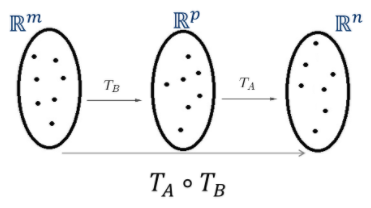
\includegraphics[scale=0.5]{comp-trans.png}
\end{center}

Would imply that $A$ is $n\times p$, $B$ is $p\times m$, and $AB$ is $n\times m$.
Can define the following:

\[\boxed{\text{The $i^{th}$ column of the matrix $AB$ is the matrix-vector product $A$($i^{th}$ column of the matrix $B$)}}\]

\subsection{Proofs}

\textbf{\textit{Claim:}} The product of 2 invertible matrices must be an invertible matrix.\newline
\textbf{\textit{Proof:}} Given that $(AB)(AB)^{-1}=I_n$:

\begin{align*}
    &(AB)(AB)^{-1}=I_n\\
    &A(B(AB)^{-1})=I_n\\
    &A^{-1}A(B(AB)^{-1})=A^{-1}I_n\\ 
    &B(AB)^{-1}=A^{-1}\\ 
    &B^{-1}B(AB)^{-1}=B^{-1}A^{-1}\\
    &(AB)^{-1}=B^{-1}A^{-1}
\end{align*}

\noindent\textbf{\textit{Claim:}} If $(AB)^{-1}$ exists, then $A$ and $B$ are both invertible.\newline
\textbf{\textit{Proof:}} Given that $(AB)(AB)^{-1}=I_n$ and $(AB)^{-1}(AB)=I_n$:

\begin{align*}
    &A(B(AB)^{-1})=I_n\\ 
    &((AB)^{-1}A)B=I_n\\
    &\boxed{\therefore\;\exists\;A^{-1},\:B^{-1}\in \R^n}
\end{align*}

\subsection{Properties}

\begin{itemize}
    \item Associativity: $(AB)C=A(BC)$
    \item Distribution: $A(B+C)=AB+BC$
    \item Respects scalar multiplication: $(kA)B=k(AB)=A(kB)$ 
\end{itemize}


\section{Transposes, Permutations, Spaces}
\subsection{Permutations}

Function to make row exchanges. Elimination with row exchanges:

\[A=LU\implies PA=LU\]

Works for any invertible $A$.

\[P=\text{identity with reordered rows (exchanges)}\]

Count of possible reorderings ($n\times n$ permutations): $n! = n(n-1)\cdots 3(2)(1)$.

\[\boxed{P^{-1}=P^T\text{ and }P^TP=I}\]

Defining a transpose, or flip over diagonal:

\[(A^T)_{ij}=A_{ji}\]

For symmetric matrices, transpose does not cause change; $A^T=A$. If two rectangular matrices $R^T$ and $R$
give a square matrix, then $R^TR$ is always symmetric.

\[\boxed{(R^TR)^T=R^TR^{TT}=R^TR}\]

\subsection{Vector Spaces and Subspaces}

Examples: $\R^2$ is all vectors in 2D space, $x-y$ plane: $\begin{bmatrix}3\\2\end{bmatrix}$.
$\R^3$ is all vectors with 3 components. All combinations of vectors in $\R^n$ yield a result in that space $\R^n$.

\[\boxed{\R^n\text{ is all column vectors with $n$ components.}}\]

The origin exists to allow for scalar multiplication and addition of vectors. Every vector space has a $\vec{0}$.

\subsubsection{Subspaces}

If a vector space is defined as 1st quadrant in $\R^2$, then multiplying by a negative scalar $k$ 
removes the result from that space, so it is not \textbf{closed} under that operation, so this is not a vector space. 
Vector space must be closed under linear combinations. Thus, subspace in $\R^2$ is all multiples of that vector, a line and the line must go through $\vec{0}$.
Every subspace must contain $\vec{0}$.\newline

Subspaces of $\R^2$:
\begin{itemize}
    \item All of $\R^2$
    \item Any line through $\vec{0}_2$ or $L$
    \item Just $\vec{0}_2$ or $Z$
\end{itemize}

Similarly, for $\R^3$ can have $\R^3$, plane, line, $\vec{0}_3$.\newline

Given $A=\left[\begin{array}{ll}
    1 & 3 \\
    2 & 3 \\
    4 & 1\end{array}\right]$, all linear combinations of these columns form a subspace. 
This is called \textbf{column space}, $C(A)$. This would form a plane in $\R^3$. Thus, the column space is a subspace.

\section{Image and Kernel}
\subsection{Defining Image and Kernel}

\subsubsection{Image}

Of a function, the set of vectors in the codomain hit by the domain.
The image of a function $f:\;\R^m\rightarrow \R^n$ is:

\[\boxed{
    \mathrm{Im}(f)=\{\vec{y}\in \R^n | \exists\;\vec{x}\in \R^m\text{ s.t. }f(\vec{x})=\vec{y}\}
}\]

Similar in concept to the range of a function in non-linear context.

\subsubsection{Kernel}

Srt of vectors in the domain that are mapped to $\vec{0}$ in the codomain.
Kernel of a function $f:\;\R^m\rightarrow \R^n$ is:

\[\boxed{
    \mathrm{Ker}(f)=\{\vec{x}\in \R^m | f(\vec{x})=\vec{0}\}
}\]

Analogous to the roots/zeros of a polynomial.

\subsection{Examples}

Following linear transformation's image lives in $\R^2$:

\[T(\vec{x})=\left(\begin{array}{cc}
    1 & 1 \\
    -1 & 1
    \end{array}\right) \vec{x}\]

Following linear transformation's image forms a plane that is
$\R^2$:

\[T(\vec{x})=\left(\begin{array}{cc}
    1 & -1 \\
    0 & 2 \\
    2 & 2
    \end{array}\right) \vec{x}\]

\subsection{Span}

If $A$ is an $n\times m$ matrix, then image of $T(\vec{x})=A\vec{x}$ is set of all vectors in $\R^n$
that are linear combinations of column vectors of $A$.\\

\noindent
Thus, the span of a set of $n$ vectors is all linear combinations of those vectors:

\[\boxed{
    \mathrm{span}(\vec{v}_1,\vec{v}_2,\cdots,\vec{v}_n)=\{\sum c_i\vec{v}_i | c_i\in\R\}
}\]

So the span of column vectors of $A$ is the image of the associated linear transformation.

\subsection{Kernel}

Kernel amounts to finding solutions to $A\vec{x}=\vec{0}$. Kernels are closed under linear combinations.
Kernel can never be empty set, it always holds true that $T(\vec{0})=\vec{0}$.

\subsection{Invertible Linear Transformations}

Main conclusions about image and kernel:

\begin{itemize}
    \item Kernel is always (trivially) $\{\vec{0}\}$, else would imply dependance and therefore singularity in the associated matrix $A$
    so $\boxed{\mathrm{ker}(T)=\{\vec{0}\}}$
    \item Image is always the space $\R^n$ if associated matrix $A$ is $n\times n$, so $\boxed{\mathrm{Im}(T)=\R^n}$
\end{itemize}

\section{Subspaces and Basis}
\subsection{Image and Kernel}

If $T:\;\R^m\rightarrow \R^n$ then $\mathrm{Im}(T)\subset \R^n$ and
$\mathrm{ker}(T)\subset \R^m$ because the associated matrix $A$ is $n\times m$ in dimension.\newline

\noindent
Both are closed under linear combinations:
\begin{itemize}
    \item If $\vec{y_1},\vec{y_2}\in \mathrm{Im}(T)$ then $a \vec{y}_{1}+b \vec{y}_{2} \in \mathrm{Im}(T)$ as well
    \item If $\vec{x_1},\vec{x_2}\in \mathrm{Ker}(T)$ then $a\vec{x_1}+b\vec{x_2}\in \mathrm{Ker}(T)$ as well
\end{itemize}

\subsection{Subspaces}

Collection of vectors in $\R^n$ is called a subspace in $\R^n$ if collection is nonempty and closed under linear combinations.
Examples (and counterexamples):

\begin{itemize}
    \item $W=\left\{\left(\begin{array}{c}
        3 s \\
        2+5 s
        \end{array}\right) \mid s \in \mathbb{R}\right\} \subset \mathbb{R}^{2}$
        is not a subspace because $\vec{0}$ is not contained within the set, so not closed under linear combinations
    \item $W=\left\{\left(\begin{array}{l}
        x_{1} \\
        x_{2} \\
        x_{2}
        \end{array}\right) \mid 2 x_{1}+x_{2}-x_{3}=0\right\}$ is a subspace due to matrix representation and 
        the image of this matrix containing $\vec{0}$ due to $T(\vec{0}=\vec{0})$
\end{itemize}

\noindent
$\R^2$ is not a subspace of $\R^3$ because though a plane can be drawn in $\R^3$, its components will be of the form
$\begin{bmatrix}x\\ y\\k\end{bmatrix}$, where $k$ is fixed. Since $\R^3$ vectors always have 3 coordinates, they can't represent $\R^2$.
$\R^2$ can only be represented by $\R^2$ vectors. Thus, $R^n$ is not a subspace of $\R^{n+1}$.\\

\noindent
\textbf{\textit{Claim:}} Span of a set of vectors in $\R^n$ is a subspace of $\R^n$.\\
\textbf{\textit{Proof:}}\\
Let $S=\{\vec{v_1},\vec{v_2},\cdots\vec{v_m}\}$. Let $\vec{w},\vec{y}\in \mathrm{span}(S)$.
Thus, $\vec{w}=\sum c_i\vec{v_i}$ and $\vec{y}=\sum d_i\vec{v_i}$ where $d_i,c_i\in \R$.

\begin{align*}
    a\vec{w}+b\vec{y}&=a\sum c_i\vec{v_i}+b\sum d_i\vec{v_i}\\
    &=\sum a c_{i} \vec{v}_{i}+\sum b d_{i} \vec{v}_{i}\\
    &=\sum\left(a c_{i}+b d_{i}\right) \vec{v}_{i} \in \operatorname{span}(S)
\end{align*}

\noindent
List of subspaces in $\R^2$ would be $\R^2$, $\{t\vec{v}\mid t\in\R\}$, $\{\vec{0}\}$.

\subsection{Intersection and Union}

If $V$ and $W$ are collections of vectors in $\R^n$:
\begin{itemize}
    \item $V \cap W=\{\vec{x} \mid \vec{x} \in V \text { and } \vec{x} \in W\}$ is the intersection
    \item $V \cup W=\{\vec{x} \mid \vec{x} \in V \text { or } \vec{x} \in W\}$ is the union
\end{itemize}

\subsection{Redundant Vectors}

If for some transformation $T$ there exists the following:

\[\operatorname{im}(T)=\operatorname{span}\left\{\left(\begin{array}{l}
    1 \\
    1 \\
    1
    \end{array}\right),\left(\begin{array}{l}
    2 \\
    2 \\
    2
    \end{array}\right),\left(\begin{array}{l}
    1 \\
    2 \\
    3
    \end{array}\right),\left(\begin{array}{l}
    2 \\
    3 \\
    4
    \end{array}\right)\right\}\]

There are redundant vectors in this case. The minimum number of vectors in the span is 2, 
for $\vec{0}$ cannot be produced then. With 3 vectors in $\R^3$, any one can be the result of linear combinations of the other 2.
So, it would be appropriate to say that:

\[\operatorname{im}(T)=\left\{\left(\begin{array}{l}
    1 \\
    1 \\
    1
    \end{array}\right),\left(\begin{array}{l}
    1 \\
    2 \\
    3
    \end{array}\right)\right\}\]

These are then \textbf{linearly independent}. This set forms a \textbf{basis} for that set of vectors.
Thus, the basis can be found for any matrix. The basis of $I_n$ is then $\{\vec{e}_1,\vec{e}_2\cdots \vec{e}_n\}$.

\subsection{Intersection and Union}

\begin{framed}
    \noindent If $V$ and $W$ are subspaces of $\R^n$, then $V\cup W$ 
    is a subspace of $\R^n$ and $V\cap W$ is \textbf{not} a subspace of $\R^n$.
\end{framed}

\noindent
An intersection is the items contained in both sets, so $\vec{0}\in V\cap W$.
If $\vec{v},\vec{w}\in V\cap W$, then $\vec{v},\vec{w}\in V$ and $\vec{v},\vec{w}\in W$. This means that
$\vec{v}+\vec{w}\in V$ and $\vec{v}+\vec{w}\in W$ so $\vec{v}+\vec{w}\in V\cap W$.
Similarly, if some $k\vec{v}\in V\cap W$ where $k\in \R$ then $k\vec{v}\in V$ and $k\vec{v}\in V$. 
Thus, $V\cap W$ is a subspace of $\R^n$.\\

\noindent
The union is the items contained in either set.
If $V=\mathrm{span}(\vec{e}_2)$ and $W=\mathrm{span}(\vec{e}_1)$, then let $\vec{y}=\begin{bmatrix}0\\ y\end{bmatrix}\in V$
and $\vec{x}=\begin{bmatrix}x\\ 0\end{bmatrix}\in W$. Thus, $\vec{y},\vec{x}\in V\cup W$. However,
$a\vec{x}+b\vec{y}\notin V\cup W$ where $a,b\in \R$.

\section{Basis of a Kernel}
\subsection{Example}

Let $A=\begin{bmatrix}1&4&7\\ 2&5&8\\3&6&9\end{bmatrix}$. Finding the basis:

\[
    \mathrm{rref}(A)=
     \begin{bmatrix}1&0&-1\\ 0&1&2\\0&0&0\end{bmatrix}
\] 

Since there is redundance, a possible expression of the basis of $A$:

\[\mathfrak{B}=\left\{\begin{bmatrix}1\\2\\3\end{bmatrix},\begin{bmatrix}4\\5\\6\end{bmatrix}\right\}\]

When finding kernel, must solve $A\vec{x}=\vec{0}$. So with $[\mathrm{rref}(A)|\vec{0}]$:

\[\vec{x}=\begin{bmatrix}t\\ -2t\\t\end{bmatrix}=t \begin{bmatrix}1\\-2\\1\end{bmatrix}\]

Thus,

\[\mathrm{ker}(A)=\left\{t\begin{bmatrix}1\\-2\\1\end{bmatrix}\bigg|\;t\in \R\right\}\]

\noindent
Subsequently, the basis of the kernel of $A$ can be represented as $\mathfrak{B}=\left\{\begin{bmatrix}1\\-2\\1\end{bmatrix}\right\}$.

\noindent
Equivalent statements for $\left\{\vec{v}_{1}, \vec{v}_{2}, \vec{v}_{3}, \ldots, \vec{v}_{m}\right\}$ being linearly independent:
\begin{itemize}
    \item None of the vectors are redundant
    \item Only relation is trivial
    \item Kernel of $\left(\begin{array}{cccc}
        \mid & \mid & & \mid \\
        \vec{v}_{1} & \vec{v}_{2} & \ldots & \vec{v}_{m} \\
        \mid & \mid & & \mid
        \end{array}\right)$ is trivial
    \item Rank of $\left(\begin{array}{cccc}
        \mid & \mid & & \mid \\
        \vec{v}_{1} & \vec{v}_{2} & \ldots & \vec{v}_{m} \\
        \mid & \mid & & \mid
        \end{array}\right)$ is $m$
    \item If $m=n$ then $\left(\begin{array}{cccc}
        \mid & \mid & & \mid \\
        \vec{v}_{1} & \vec{v}_{2} & \ldots & \vec{v}_{m} \\
        \mid & \mid & & \mid
        \end{array}\right)$ reduces to $I_n$
\end{itemize}

\section{Dimension}
\subsection{Rank and independence}

If $\{\vec{v}_1,\vec{v}_2,\cdots ,\vec{v}_m\}$ is a collection if independent vectors then

\[
\left(\begin{array}{ccccc}
\mid & \mid & \mid & & \mid \\
\vec{v}_{1} & \bar{v}_{2} & \bar{v}_{3} & \ldots & \bar{v}_{m} \\
\mid & \mid & \mid & & \mid
\end{array}\right)
\]

must have a rank of $m$. This is because row reducing the matrix corresponds to the following relation:

\[c_1\vec{v}_1+c_2\vec{v}_2+c_3\vec{v}_3+\dots +c_m\vec{v}_m=\vec{0}\]

\noindent
Also, $m\leq n$ where $n$ is the number of rows in each column vector, in order to have linear independence for this set.

\subsection{Dimension}

Considering an $xy$-plane in $\R^3$:

\[V=\left\{\begin{bmatrix}s\\t\\0\\ \end{bmatrix}\Bigg| s,t \in \mathbb{R} \right\}\]

The basis of this set contains 2 vectors (e.g. dimension of 2), with example being:

\[\mathfrak{B}=\left\{\begin{bmatrix}1\\0\\0 \end{bmatrix} , \begin{bmatrix} 0\\1\\0 \end{bmatrix} \right\}\]

\begin{framed}
    If $V$ is a subspace of $\R^n$ and $\mathfrak{B}$ and $\mathfrak{C}$ are two bases of $V$, then
    $\mathfrak{B}$ and $\mathfrak{C}$ contain the same number of vectors.
\end{framed}

\textbf{Dimension} of a subspace is number of vectors in the basis.

\subsubsection{Example}

Considering the following matrix:

\[A=\begin{bmatrix}
    1&2&0&1&2\\
    1&2&0&2&3\\
    1&2&0&3&4\\
    1&2&0&4&5\\
    \end{bmatrix}\]

By discounting the redundant vectors, a possible basis for $\mathrm{Im}(A)$:

\[\mathfrak{B}_\mathrm{image}=\left \{\begin{bmatrix} 1\\1\\1\\1 \end{bmatrix},\begin{bmatrix}1\\2\\3\\4 \end{bmatrix} \right\}\]

So the dimension of $\mathrm{Im}(A)$ is 2.
Finding a basis for $\mathrm{ker}(A)$ is the same as solving $A\vec{x}=\vec{0}$:

\[\mbox{ker}(A)=\left\{\begin{bmatrix}-2s-w\\ s\\t\\-w\\w \end{bmatrix} \Bigg| s,t,w\in\mathbb{R} \right\}=
\left\{s\begin{bmatrix}-2\\1\\0\\0\\0\\\end{bmatrix}+t\begin{bmatrix}0\\0\\1\\0\\0\\\end{bmatrix}+w\begin{bmatrix}-1\\0\\0\\-1\\1\\\end{bmatrix}\Bigg|s,t,w\in\mathbb{R}\right\}\]

So the basis for $\mathrm{ker}(A)$:

\[\mathfrak{B}_\mathrm{kernel}=\left\{\begin{bmatrix}-2\\1\\0\\0\\0\\ \end{bmatrix}, \begin{bmatrix} 0\\0\\1\\0\\0\\ \end{bmatrix}, \begin{bmatrix}-1\\0\\0\\-1\\1\\ \end{bmatrix} \right\}\]

And dimension of $\mathrm{ker}(A)$ is 3.
However, it is shown that $\mathrm{rref}(A)$ gives dimension of \textbf{image and kernel}.

\subsection{Rank-Nullity Theorem}

\begin{framed}
    \begin{itemize}
        \item If $T$ is a linear transformation, 
        then \\$\mathrm{dim}(\mathrm{Im}(T))+\mathrm{dim}(\mathrm{ker}(T))=\text{dimension of domain of }T$
        \item If $A$ is a matrix, then $\mathrm{rank}(A)+\mathrm{nullity}(A)=\text{number of columns of }A$
        \item In a linear system, 
        \\$\text{number of leading variables}+\text{number of free variables}=\text{total number of variables}$
    \end{itemize}
\end{framed}

Considering non-invertible matrices $A$ and $B$, let $AB$ be invertible.
It must hold true that $\mathrm{ker}(B)=\{\vec{0}\}$. If the dimensions of $B$ are $p\times n$,
$\mathrm{Im}(B)$ is a subspace of $\R^p$ has dimension $n$. This means that it is a vertically rectangular
matrix with $n\leq p$. Thus, $A$ is $n\times p$ so it is horizontally rectangular.

\section{Coordinates}
\subsection{Coordinate vectors}

For example, the basis of $xy$ plane can be:

\[\mathfrak{B}=\left\{\begin{bmatrix} 1\\1\\0\\ \end{bmatrix}, \begin{bmatrix}1\\-1\\0\\ \end{bmatrix}\right\}\]

To form $\begin{bmatrix}1\\ 0\\0\end{bmatrix}$ with this basis, can do $\begin{bmatrix} 1\\0\\0\\ \end{bmatrix}=\frac{1}{2}\begin{bmatrix} 1\\1\\0\\ \end{bmatrix}+\frac{1}{2}\begin{bmatrix}1\\-1\\0\\ \end{bmatrix}$.
The coefficients used form the following vector:

\[\begin{bmatrix}\frac{1}{2}\\ \frac{1}{2}\end{bmatrix}\]

Known as \textbf{$\mathfrak{B}$-coordinate vector}.
Notation:

\[\left[\begin{bmatrix} 1 \\ 0 \\ 0 \end{bmatrix} \right]_\mathfrak{B}=\begin{bmatrix} \frac{1}{2} \\ \frac{1}{2} \\ \end{bmatrix} \]

\begin{framed}
\noindent
Generally, given $\mathfrak{B}=\left\{ \vec v_1, \vec v_2, \vec v_3, \dots, \vec v_m \right\}\subset \mathbb{R}^n$
is linearly independent, then $[\vec{v}_i]_{\mathfrak{B}}=\vec{e}_i\in\R^m$.
\end{framed}

This is because row-reducing the matrix of $\mathfrak{B}$ gives $\mathrm{rref}(A)$ where $A$ is this matrix. Given the same
$\mathfrak{B}$, can find the components of $\vec{w}$:

\[\left[\vec w \right]_\mathfrak{B}=\begin{bmatrix}c_1\\c_2\\ \vdots\\ c_m\end{bmatrix}\]
\[\vec{w}=c_{1} \vec{v}_{1}+c_{2} \vec{v}_{2}+\cdots+c_{m} \vec{v}_{m}\]

Thus,

\[\vec w = \begin{bmatrix}|&|&\dots&|\\ \vec v_1 &\vec v_2 & \dots &\vec v_m\\  |&|&\dots&| \end{bmatrix}\begin{bmatrix}c_1\\c_2\\\vdots\\c_m\end{bmatrix}\]

Matrix is called change of basis matrix $S$. A standard basis is given as $\vec{e}_1,\vec{e}_2,\cdots$. A nonstandard basis is not of this form.

\subsection{B-matrix}

If $A$ is $n\times n$ and $T(\vec{x})=A\vec{x}$ where $T:\R^n\rightarrow \R^n$, then there exists a matrix $B$ such that
$\left[T(\vec x)\right]_\mathfrak{B}=B\left[\vec x\right]_\mathfrak{B}$. This is called the $\mathfrak{B}-matrix$.
If $\vec{v}_i\in \mathfrak{B}$, then $[\vec{v}_i]_\mathfrak{B}=\vec{e}_i$.\\

\noindent
This means that 
$\left[T(\vec v_i)\right]_\mathfrak{B}=B\left[\vec v_i \right]_\mathfrak{B}=B\vec e_i$, so 
\textbf{the $i^{\mathrm{th}}$column of $B$ must be $[T(\vec{v}_i)]_\mathfrak{B}$}.\\

\noindent
Multiple ways to calculate $\mathfrak{B}$-matrix of $T$, considering $T$ to be a projection
onto $y=\frac{x}{3}$:

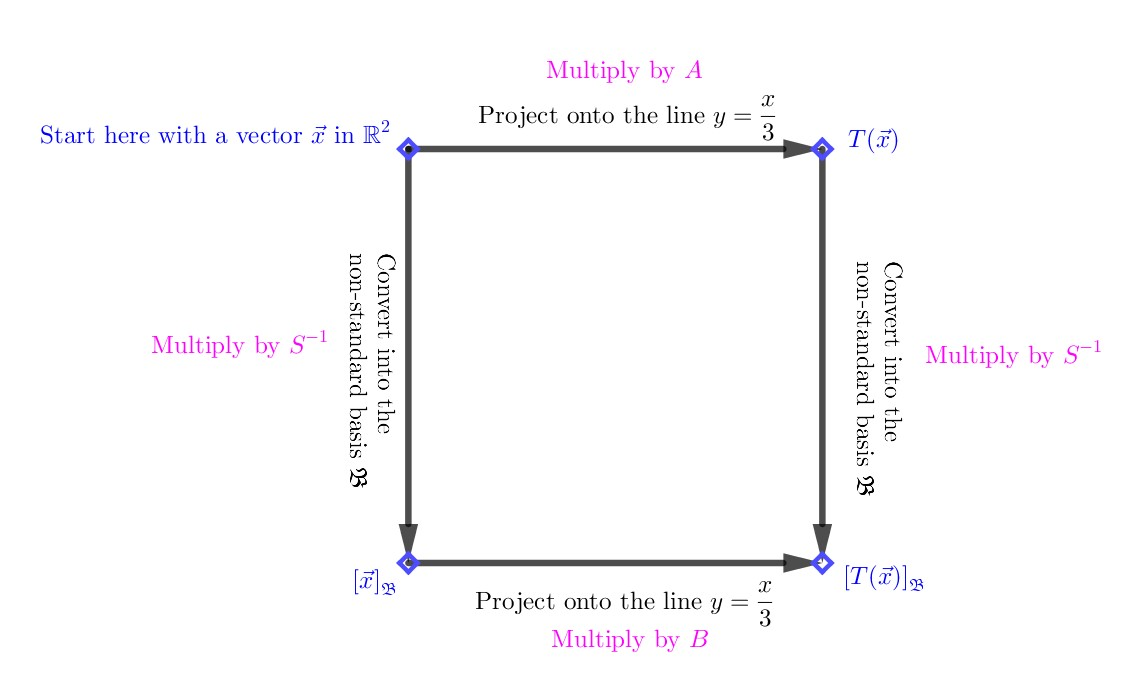
\includegraphics[scale=0.5]{CommutativeDiagram2.jpg}

Means that multiple ways to get to $[T(\vec{x})]_\mathfrak{B}$.
When following $\vec{x}$ and going right and down:

\[S^{-1}\left(A\vec x\right)=S^{-1}A\vec x=\left[T(\vec x) \right]_\mathfrak{B}\]

Going down and right:

\[B\left(S^{-1}\vec x\right)=BS^{-1} \vec x=\left[T(\vec x )\right]_\mathfrak{B}\]

Thus,

\begin{align*}
S^{-1}A=BS^{-1}\\
\boxed{S^{-1}AS=B}
\end{align*}

If this is satisfied, then $A$ is similar to $B$ or $A\sim B$.

\section{Determinants}
\subsection{Introduction to Determinant}

Can define the $2\times 2$ determinant as a function $D:\mathbb{M}_{2\times2}\rightarrow R$.
It can be observed that $2\times 2$ matrix $A$ is only invertible if $D(A)=ad-bc\neq 0$.

\subsection{Cross-Product}

Given $\begin{bmatrix}a\\ c\end{bmatrix}$ and $\begin{bmatrix}b\\ d\end{bmatrix}$, the cross
product is defined as the $\R^3$ vector $D(A)\vec{e}_3=(ad-bc)\vec{e}_3$. The direction
of this vector is the sign of $\mathrm{det}(A)$.

\noindent
Can visualize using right hand rule: if sweeping index into middle is appropriate for the vectors,
then the direction of thumb is cross-product direction (positive). Otherwise, sign is negative.

\subsubsection{Algorithm}

For $\vec{v}=\begin{bmatrix}v_x\\ v_y\\ v_z\end{bmatrix}$ and $\vec{w}=\begin{bmatrix}w_x\\ w_y\\ w_z\end{bmatrix}$:

\[\boxed{\vec{v}\times\vec{w}=c_z\vec{e}_1+c_y\vec{e}_2+c_z\vec{e}_z}\]

Following through, to calculate each component ignore the desired row and perform cross-product on remaining matrix:

\[c_x=\begin{bmatrix}v_y\\ v_z\end{bmatrix}\times \begin{bmatrix}w_y\\ w_z\end{bmatrix}=v_yw_z-v_zw_z\]

The $y$ component is done as $bc-ad$ compared to $ad-bc$.

\[c_y=\begin{bmatrix}v_x\\ v_z\end{bmatrix}\times \begin{bmatrix}w_x\\ w_z\end{bmatrix}=w_xv_z-w_zv_x\]

\[c_z=\begin{bmatrix}v_y\\ v_z\end{bmatrix}\times \begin{bmatrix}w_y\\ w_z\end{bmatrix}=v_xw_y-v_yw_x\]

\subsection{Determinant Theory}

Considering $A=\begin{bmatrix}|&|&| \\\vec v_1 & \vec v_2 &\vec v_3 \\ |&|&| \\ \end{bmatrix}$,
say it is singular such that $\vec{v}_3\in \mathrm{span}\{\vec{v}_1,\vec{v}_2\}$. Because it is assumed that
$\vec{v}_1,\vec{v}_2$ are linearly independent, then $\mathrm{span}\{\vec{v}_1,\vec{v}_2\}$ is perpendicular to 
$\vec{v}_1\times \vec{v}_2$ by definition. Thus, $\boxed{(\vec{v}_1\times\vec{v}_2)\cdot \vec{v}_3=0}$.
If $\vec{v}_1,\vec{v}_2$ are not linearly independent, then this is still 0 because the cross-product (area of parallelogram made by vectors)
is still 0.

\noindent
If $\vec{v}_1,\vec{v}_2,\vec{v}_3$ are linearly independent, then $(\vec{v}_1\times\vec{v}_2)\cdot \vec{v}_3\neq0$.

\[\boxed{D(A)=\mathrm{det}(A)=(\vec{v}_1\times\vec{v}_2)\cdot \vec{v}_3}\]

\noindent
The sub-matrices used when computing cross-products are \textbf{minors}.
Can rewrite determinant:

\[\boxed{\det A= a_{1,3}\left|A_{1,3}\right|-a_{2,3}\left|A_{2,3}\right|+a_{3,3}\left|A_{3,3}\right|}\]

Must use following rule for the sign of constant terms $a_{m,n}$ (dot product):

\[\begin{bmatrix}+&-&+\\-&+&-\\+&-&+\end{bmatrix}\]

\subsection{Rules}

Determinant of $n\times n$ follows recursively:

\[\boxed{\mbox{det}A=a_{1,1}\left|A_{1,1}\right|-a_{1,2}\left|A_{1,2}\right|+a_{1,3}\left|A_{1,3}\right|+\dots\pm a_{1,n}\left|A_{1,n}\right|}\]

\noindent
Rules:
\begin{itemize}
    \item Swapping rows multiplies determinant by -1
    \item Multiplying row by $m$ scales determinant by $m$
    \item Replacing row with sum of row and multiple of another does not change determinant
    \item If $A$ and $B$ are $n\times n$, then $\mathrm{det}(AB)=\mathrm{det}(A)\mathrm{det}(B)$
    \item Cramer's rule: If $A\vec{x}=\vec{b}$ is a linear system with invertible $A$ then $\vec{x}$ components can be determined
    from $x_i=\frac{\mathrm{det}(A-_{b,i})}{\mathrm{det}(A)}$ where $A-_{b,i}$ replaces $i^{\mathrm{th}}$ column of $A$ with $\vec{b}$
\end{itemize}

\section{Intro to Dynamical Systems}
\subsection{Dynamical Systems and Eigenvectors}

In general, a discrete dynamical system can be modeled as:

\[\boxed{\vec{x}(t+1)=A\vec{x}(t)}\]

where the transformation undergone by the system is $\vec{x}(t)\rightarrow\vec{x}(t+1)$ with matrix $A$.
Additionally, note that $\vec{x}(t)=\begin{bmatrix}c(t)\\r(t)\end{bmatrix}$ where $c(t)$ and $r(t)$ are some closed formulas.

Finding $\vec{x}(t)$ for an arbitrary integer $t>0$:

\[\boxed{\vec{x}(t)=A^t\vec{x}(0)=A^t\vec{x}_0}\]

Repeat definition of eigenvector from below:

\begin{framed}
    If $A$ is an $n\times n$ matrix, an eigenvector of $A$ is a nonzero vector $\vec{v}$
    that has the property that $\vec{v}$ and $A\vec{v}$ are parallel.
    Same as saying that $A\vec{v}=\lambda\vec{v}$, so $\lambda$ is an eigenvalue.
\end{framed}

\subsection{Dynamical Systems Example}

Following equations model transformation from $t$ to $t+1$:

\[\boxed{
    \begin{array}{l}
        c(t+1)=0.86 c(t)+0.08 r(t) \\
        r(t+1)=-0.12 c(t)+1.14 r(t)
        \end{array}
}\]

Is discrete dynamical linear system: changed over discrete time interval and dynamic as
variables change according to $t$. As a matrix-vector equation:

\[\left(\begin{array}{cc}
    0.86 & 0.08 \\
    -0.12 & 1.14
    \end{array}\right)\left(\begin{array}{l}
    c(t) \\
    r(t)
    \end{array}\right)=\left(\begin{array}{l}
    c(t+1) \\
    r(t+1)
    \end{array}\right)\]

$\vec{x}(t)=\left(\begin{array}{l}c(t) \\r(t)\end{array}\right)$
is the \textbf{state vector} at time $t$. $\vec{x}(0)=\left(\begin{array}{l}c_{0} \\r_{0}\end{array}\right)$
is the \textbf{initial state vector}. Calculating arbitrary state vector:

\[\left(\begin{array}{cc}
    0.86 & 0.08 \\
    -0.12 & 1.14
    \end{array}\right)^{t} \vec{x}_{0}=\vec{x}(t)\]

In this example, $c(t)=(100) 1.1^{t}$ and $r(t)=(300) 1.1^{t}$, so next
state vector is 1.1 times the current. However, for $\vec{x}_{0}=\left(\begin{array}{c}1000 \\1000\end{array}\right)$
there exists no such scalar pattern. Can use the basis of 2 (scalar pattern respected) vectors:

\[\mathfrak{B}=\left\{\left(\begin{array}{l}
    100 \\
    300
    \end{array}\right),\left(\begin{array}{l}
    200 \\
    100
    \end{array}\right)\right\}\]

Writing this state vector as a lin. combination:

\[\left(\begin{array}{l}
    1000 \\
    1000
    \end{array}\right)=2\left(\begin{array}{l}
    100 \\
    300
    \end{array}\right)+4\left(\begin{array}{l}
    200 \\
    100
    \end{array}\right)\]

After applying coefficient matrix to both sides and simplifying:

\[\left(\begin{array}{cc}
    0.86 & 0.08 \\
    -0.12 & 1.14
    \end{array}\right)^{t}\left(\begin{array}{c}
    1000 \\
    1000
    \end{array}\right)=2(1.1)^{t}\left(\begin{array}{c}
    100 \\
    300
    \end{array}\right)+4(0.9)^{t}\left(\begin{array}{c}
    200 \\
    100
    \end{array}\right)\]

Thus,

\[\begin{array}{l}
    c(t)=200(1.1)^{t}+800(0.9)^{t} \\
    r(t)=600(1.1)^{t}+400(0.9)^{t}
    \end{array}\]

Different trajectories for various initial state vectors:

\begin{center}
    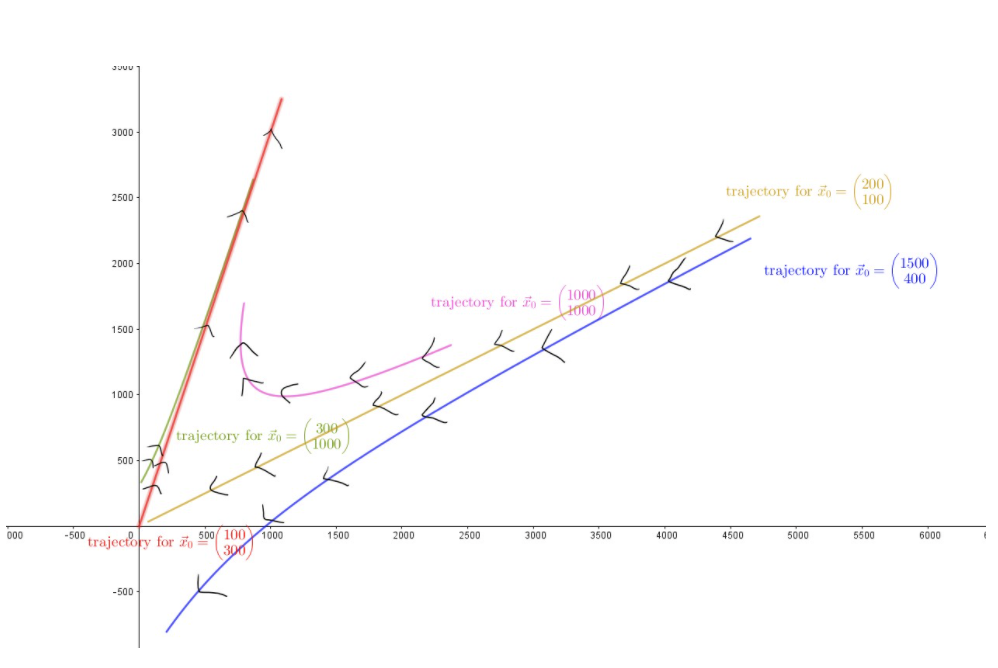
\includegraphics[scale=0.5]{state-vectors.png}
\end{center}

Called a \textbf{phase portrait} for a discrete dynamical system.
Indicates performing of system based on initial states.
The 2 state vectors in the basis are \textbf{eigenvectors}.

\begin{framed}
    If $A$ is an $n\times n$ matrix, an eigenvector of $A$ is a nonzero vector $\vec{v}$
    that has the property that $\vec{v}$ and $A\vec{v}$ are parallel.
    Same as saying that $A\vec{v}=\lambda\vec{v}$, so $\lambda$ is an eigenvalue.
\end{framed}

If there exists an $n\times n$ matrix $A$ with $\lambda=0$, then kernel of $A$ must be nontrivial
because $A\vec{v}=\vec{0}=0\vec{v}$, therefore $A$ is singular.

\section{Eigenvalue of a Matrix}
\subsection{Eigenvalue for rotation transformation}

\textbf{\textit{Claim:}} 
If $0< \theta <2\pi$ then transformation $R_\theta : \R^2\rightarrow \R^2$ only has an eigenvector when $\theta=\pi$ (when $\lambda=-1$).
\newline \noindent
\textbf{\textit{Proof:}}
\noindent
The matrix is $A=\begin{bmatrix}\cos\theta & -\sin\theta\\\sin\theta & \cos\theta\end{bmatrix}$. Following by the definition of an eigenvector:

\[
    \begin{aligned}
        A \tb{v} &=\lambda v \Longleftrightarrow \\
        A \tb{v}-\lambda \tb{v} &=\overrightarrow{0} \Longleftrightarrow \\
        A \tb{v}-\lambda(I \tb{v}) &=\overrightarrow{0} \Longleftrightarrow \\
        A \bar{v}-(\lambda I) \tb{v} &=\overrightarrow{0} \Longleftrightarrow \\
        (A-\lambda I) \tb{v} &=\overrightarrow{0} \Longleftrightarrow \\
            \operatorname{det}(A-\lambda I)&=0
        \end{aligned}    
\]

Thus,

\[
    \begin{aligned}
        \operatorname{det}(A-\lambda I) &=0 \\
        \operatorname{det}\left(\begin{array}{cc}
        \cos \theta-\lambda & -\sin \theta \\
        \sin \theta & \cos \theta-\lambda
        \end{array}\right) &=0 \\
        \lambda^{2}-2 \lambda \cos \theta+\cos ^{2} \theta+\sin ^{2} \theta &=0 \\
        \lambda^{2}-2 \lambda \cos \theta+1 &=0
        \end{aligned}    
\]

The discriminant of this quadratic ($b^2-4ac$) is $4\cos^2\theta-4$, so for a real solution $4\cos^2\theta-4\geq 0$. It then follows
that:

\begin{align*}
    4\cos^2\theta-4&\geq 0\\
    \cos^2\theta&\geq 1\\
    \cos^2\theta&=\pm 1\\
    \theta&=\pi
\end{align*}

Note that because $(A-\lambda I)\tb{v}=\tb{0}$ implies a nontrivial kernel for $A-\lambda I$, $\mathrm{det}(A-\lambda I)=0$.

\subsection{Characteristic Polynomials}

Characteristic polynomial is for $\mathrm{det}(A-\lambda I)$ with variable $\lambda$: 

\[\boxed{P_A(\lambda)=\mathrm{det}(A-\lambda I)}\]

General polynomial for $A=\begin{bmatrix}a&b\\c&d\end{bmatrix}$:

\[
    \begin{aligned}
        p_{A}(\lambda) &=\operatorname{det}(A-\lambda I) \\
        &=\operatorname{det}\left(\begin{array}{cc}
        a-\lambda & b \\
        c & d-\lambda
        \end{array}\right) \\
        &=(a-\lambda)(d-\lambda)-b c \\
        &=\lambda^{2}-(a+b) \lambda+(a d-b c)    
    \end{aligned}
\]

Ends up that $\mathrm{tr}(A)=a+d$ and $\mathrm{det}(A)=ad-bc$:

\[\boxed{p_{A}(\lambda)=\lambda^{2}-\operatorname{tr} A \lambda+\operatorname{det} A}\]

\subsubsection{General formula}

In general, if $A$ is an $n\times n$ matrix, then

\[\boxed{p_{A}(\lambda)=(-1)^{n} \lambda^{n}+(-1)^{n-1} \operatorname{tr} A \lambda^{n-1}+\cdots+\operatorname{det} A}\]

Conjectures:
\begin{itemize}
    \item By FTLA, degree $n$ polynomial will have $n$ complex roots so at least $n$ real eigenvalues
    \item If all $n$ roots are real, then $\mathrm{tr}(A)$ is sum of eigenvalues and determinant is the product of them
    \item Since roots are either real or in complex conjugate pairs, ($a+bi$ or $a-bi$) then when $n$ is odd $A$ has at least 1 real eigenvalue
\end{itemize}

\section{Eigenvector of a Matrix}
\subsection{Eigenspace}

Kernel of a matrix always forms subspace of domain. If $\lambda$ is an eigenvalue for $A$,
kernel of $A-\lambda I$ is the \textbf{eigenspace} associated with $\lambda$ and 
this is denotes as $E_\lambda=\mathrm{ker}(A-\lambda I)$.

If $A-\lambda I$ has column vectors $\vec{v}_1$ and $\vec{v}_2$, then 
$E_\lambda=\mathrm{span}\left\{\begin{bmatrix}c_1\\c_2\end{bmatrix}\right\}$ where $c_1\vec{v}_1+c_2\vec{v}_2=\vec{0}$.

\subsection{Multiplicity}

Dimension of eigenspace $E_\lambda$ is \textbf{geometric multiplicity} of $\lambda$.
Multiplicity of root $\lambda$ is \textbf{algebraic multiplicity} in characteristic polynomial $p_A(\lambda)$.
Therefore, geometric multiplicity $\leq$ algebraic multiplicity, considering the case of $p_A(\lambda)=(\lambda-\lambda_0)^2$.

Thus, this represents a $2\times 2$ matrix which fixes one line and moves every other line, known as a shear. All lines but $x$-axis move.
Has characteristic polynomial $p_A(\lambda)=(\lambda-1)^2$, so $E_1=\mathrm{ker}\begin{bmatrix}0&k\\0&0\end{bmatrix}=\mathrm{span}\left\{\begin{bmatrix}1\\0\end{bmatrix}\right\}$.

\subsection{Eigenbasis}

Consists of the eigenvectors of the coefficient matrix. An $n\times n$ matrix needs $n$ linearly independent
eigenvectors to have an eigenbasis. This means that if $A$ has eigenvectors $\lambda_1\neq\lambda_2$, then $E_{\lambda_1}\cap E_{\lambda_2}=\left\{\vec{0}\right\}$.
This is because if some $\vec{v}\in E_{\lambda_1}$, then $A\vec{v}=\lambda_1\vec{v}$ and $A\vec{v}=\lambda_2\vec{v}$.
Thus, $(\lambda_1-\lambda_2)\vec{v}=\vec{0}$, so $\vec{v}=\vec{0}$.

\noindent
Furthermore, if $E_{\lambda_1}$ has basis $\mathfrak{E}_{\lambda_1}$ and $E_{\lambda_2}$ with $\mathfrak{E}_{\lambda_2}$, $\mathfrak{E}_{\lambda_1}\cup \mathfrak{E}_{\lambda_2}$ is linearly independent as well 
with the total elements being the sum of the number of elements in each individual basis.
Can then be concluded that:

$$
\boxed{\text{An $n\times n$ matrix has eigenbasis iff sum of geometric multiplicities of eigenvalues is $n$.}}
$$

\section{Diagonalization}
\subsection{Diagonalization and Properties}

Diagonal matrix has entries not along the main diagonal be all 0. Example:

\[A=\begin{bmatrix}1&0&0\\0&3&0\\0&0&-1\\ \end{bmatrix}\]

Characteristic polynomial ends up being

\begin{align*}
    p_A(\lambda)&=\mbox{det}\begin{bmatrix}1-\lambda&0&0\\ 0&3-\lambda&0\\ 0&0&-1-\lambda\\ \end{bmatrix}\\
    p_A(\lambda)&=(1-\lambda)(3-\lambda)(-1-\lambda)
\end{align*}

\noindent
Matrix similar to diagonal matrix is \textbf{diagonalizable}. Thus, $A$ is diagonalizable if
there exists an invertible $S$ and diagonal matrix $D$ such that $\boxed{S^{-1}AS=D}$. 
Because it is known that if $A\sim B$, $p_A(\lambda)=p_B(\lambda)$, whenever $A$ is diagonalizable, the
eigenvalues of $A$ will be diagonal entries of any diagonal matrix $A$ is similar to.

\noindent
Also note that for a diagonal matrix $D$, $D^t$ consists of all the diagonal entries $\lambda_1^t, \lambda_2^t\cdots, \lambda_n^t$:

\[D^t=\begin{bmatrix}
    \lambda_1^t&0&0&0\\
    0&\lambda_2^t&0&0\\
    0&0&\ddots&0\\
    0&0&0&\lambda_n^t\\
\end{bmatrix}\]

It then follows that if $S^{-1}AS=D$:

\begin{align*}
    S^{-1}AS&=D\\
    (S^{-1}AS)^t&=D^t\\
    (S^{-1}AS)(S^{-1}AS)(S^{-1}AS)\dots(S^{-1}AS)&=D^t\\
    S^{-1}A^tS&=D\\
    A^t&=SD^tS^{-1}\\
\end{align*}

\subsection{Diagonalization and Eigenbasis}

\textbf{A square matrix is diagonalizable if it has an eigenbasis.}

\noindent
Let the eigenbasis be $\mathfrak{E}=\left\{\tb v_1, \tb v_2, \tb v_3, \dots, \tb v_n\right\}$.
To show $A$ is diagonalizable, the $\mathfrak{E}$-matrix can be shown to be diagonal. First, let
$A$'s transformation be $T_A(\tb{x})=A\tb{x}$. The $\mathfrak{E}$-matrix is $D$. Thus, $\boxed{D[\tb x]_\mathfrak{E}=[T_A(\tb x)]_\mathfrak{E}}$.
The first column of $D$ is $[T_A(\tb{v}_1)]_\mathfrak{E}$. However, because $\mathfrak{E}$ is an eigenbasis for $A$,
it must hold true that:

\[A\tb v_1=T_A(\tb v_1)=\lambda_1 \tb v_1\]

\noindent
Thus, first column of $D$ is $[\lambda_1\tb{v}_1]_\mathfrak{E}$. Since $\lambda _1 \tb v_1=\lambda_1 \tb v_2+0\tb v_2+0\tb v_3+\dots+0\tb v_n$
as it is part of an eigenbasis, $[\lambda _1 \tb v_1]_\mathfrak{E}=\begin{bmatrix}\lambda_1\\0\\0\\ \vdots \\ 0 \end{bmatrix}$.
If repeated for all vectors in $\mathfrak{E}$, it ends up being that:

\[D=\begin{bmatrix}\lambda_1&0&0&0\\
    0&\lambda_2&0&0\\
    0&0&\ddots&0\\
    0&0&0&\lambda_n
\end{bmatrix}\]

It must also hold true that if $A$ is diagonalizable, it has an eigenbasis. It is known that:

\[S^{-1}AS=D=\begin{bmatrix}\lambda_1&0&0&0\\0&\lambda_2&0&0\\ 0&0&\ddots&0\\ 0&0&0&\lambda_n \end{bmatrix}\]

so a basis in $\R^n$ consisting of eigenvectors must be found. This is found in the columns of $S$, the change of basis matrix.
The similarity formula can be rearranged to get $AS=SD$. Thus, for the first column of $S$, $S\tb{e}_1$:

\begin{align*}
    A(S\tb e_1)&=(AS)\tb e_1\\
    &=(SD)\tb e_1\\
    &=S(D \tb e_1)\\
    &=S(\lambda_1 \tb e_1)\\
    &=\lambda_1 (S\tb e_1)\\    
\end{align*}

\noindent
This is indeed a basis as $S$ is required to be invertible.

% -------------------------------------
\end{document}